\documentclass[%
reprint,
%superscriptaddress,
%groupedaddress,
%unsortedaddress,
%runinaddress,
%frontmatterverbose, 
%preprint,
%preprintnumbers,
nofootinbib,
%nobibnotes,
%bibnotes,
 amsmath,amssymb,
aps,
%pra,
%prb,
%rmp,
%prstab,
%prstper,
%floatfix,
superscriptaddress,
showkeys,
%endfloats,
%onecolumn,
longbibliography
]{revtex4-1}

%TESTE
\usepackage{enumitem}

\usepackage{xr}
\usepackage{tabularx}
\usepackage{booktabs}
\usepackage{graphicx}% Include figure files
\usepackage{dcolumn}% Align table columns on decimal point
\usepackage{bm}% bold math
\usepackage{microtype}
\usepackage{gensymb}
\usepackage{url}
% Permitir inclusão de PDFs com versão mais alta no output (não resolve a inclusão em si)
\pdfminorversion=7
\pdfobjcompresslevel=0
% add hypertext capabilities e evitar duplicação de anchors
\usepackage[breaklinks, hidelinks, colorlinks=true,linkcolor=blue,citecolor=black,hypertexnames=false]{hyperref}
\usepackage{color, colortbl}
\usepackage[table,xcdraw]{xcolor}
%\usepackage[mathlines]{lineno}% Enable numbering of text and display math
%\linenumbers\relax % Commence numbering lines

%\usepackage[showframe,%Uncomment any one of the following lines to test 
%%scale=0.7, marginratio={1:1, 2:3}, ignoreall,% default settings
%%text={7in,10in},centering,
%%margin=1.5in,
%%total={6.5in,8.75in}, top=1.2in, left=0.9in, includefoot,
%%height=10in,a5paper,hmargin={3cm,0.8in},
%]{geometry}

%VER
% (Removido xcolor duplicado)

\makeatletter
\renewcommand\frontmatter@abstractwidth{\dimexpr0.9\textwidth\relax}
\makeatother


% \bibliographystyle{apsrev4-1}
\usepackage{algorithm}
\usepackage{algpseudocode}
\usepackage{multirow}

\makeatletter
\newcommand*{\addFileDependency}[1]{% argument=file name and extension
  \typeout{(#1)}
  \@addtofilelist{#1}
  \IfFileExists{#1}{}{\typeout{No file #1.}}
}
\makeatother

\newcommand*{\myexternaldocument}[1]{%
    \externaldocument{#1}%
    \addFileDependency{#1.tex}%
    \addFileDependency{#1.aux}%
}

\newcommand{\sm}{\scalebox{0.5}[1.0]{\( - \)}}


%VER
\makeatletter
\renewcommand\subparagraph{\@startsection{subparagraph}{5}{\parindent}%
    {3.25ex \@plus1ex \@minus .2ex}%
    {-1em}%
    {\normalfont\normalsize\bfseries}}
\makeatother

\begin{document}

\preprint{1}



\title{VessShape: Few-shot 2D blood vessel segmentation by leveraging shape priors from synthetic images}
%VessShape: Few-shot blood vessel segmentation using shape priors from synthetic data
%VessShape: Adding shape priors to neural networks for few-shot blood vessel segmentation

\author{Wesley Nogueira Galvão}
\affiliation{Department of Computer Science, Federal University of S\~ao Carlos, S\~ao Carlos, SP, Brazil}


\author{Cesar H. Comin}
\email[Corresponding author: ]{comin@ufscar.br}
\affiliation{Department of Computer Science, Federal University of S\~ao Carlos, S\~ao Carlos, SP, Brazil}

\date{\today}% It is always \today, today,
             %  but any date may be explicitly specified

\begin{abstract}

Semantic segmentation of blood vessels is a crucial task in medical image analysis, but its progress is often hindered by the scarcity of large annotated datasets and the poor generalization of models across different imaging modalities. A key aspect is the tendency of Convolutional Neural Networks (CNNs) to learn texture-based features, which limits their performance when applied to new domains with different visual characteristics. We hypothesize that leveraging the universal geometric prior of vessel-like shapes, tubular and branching structures, can lead to more robust and data-efficient models. To investigate this, we introduce VessShape, a large-scale 2D synthetic dataset designed to instill a shape bias in segmentation models. VessShape consists of images with procedurally generated tubular geometries combined with a wide variety of foreground and background textures, encouraging models to learn shape cues rather than textures. We demonstrate that a model pretrained on VessShape achieves strong few-shot segmentation performance on two real-world datasets from different domains, requiring only four to ten samples for fine-tuning. Furthermore, the model exhibits notable zero-shot capabilities, effectively segmenting vessels in unseen domains without any target-specific training. Our results indicate that pretraining with a strong shape bias can be an effective strategy to overcome data scarcity and improve model generalization in blood vessel segmentation.

\end{abstract}

\keywords{Blood vessel segmentation, shape bias, domain adaptation, few-shot learning}

\maketitle
\thispagestyle{plain}
%\ohead*{\pagemark}

\section{Introduction}
\label{sec:introduction}

The semantic segmentation of blood vessels is an active area of research, driven by the demand for precise and automated analysis of medical images in both human and animal tissues. A significant challenge in this task is the labor-intensive process of manual annotation, which requires domain expertise to create accurate segmentation masks.

This annotation bottleneck has led to a scarcity of large-scale datasets, which limits the training capacity of deep learning models. For instance, widely used public datasets such as DRIVE \cite{Staal2004} and CHASE\_DB1 \cite{Fraz2012ensemble} contain only a few dozen annotated images each. Although recent efforts have introduced new datasets \cite{jin2022fives, fhima2024lunet}, the availability of large and diverse collections remains limited. This problem is compounded by significant domain shifts between different imaging modalities, such as retinal fundus photography and cerebral cortex microscopy. Variations in texture, vessel density, and caliber hinder the ability of models trained in one domain to generalize to another.

Transfer learning is a common strategy to address these limitations. By reusing representations learned on a source domain, models can achieve better performance on a target domain, even with limited data. Techniques such as fine-tuning and domain adaptation allow models pretrained on large-scale natural image datasets, like ImageNet \cite{JiaDeng2009}, to be adapted for biomedical segmentation tasks \cite{zoetmulderDomainTaskspecificTransfer2022}.

However, a potential pitfall of standard transfer learning is the inherent bias of Convolutional Neural Networks (CNNs) toward learning texture-based features rather than geometric shapes \cite{geirhos2018, islam2021shape}. This texture bias can limit generalization across domains with different visual styles. Research has shown that models trained with an emphasis on shape cues exhibit improved performance and robustness \cite{geirhos2018}. This suggests that transferring shape representations, rather than texture-rich features, could be a more effective strategy for few-shot blood vessel segmentation.

The task of blood vessel segmentation is particularly well suited for a shape-centric approach. The fundamental geometry of blood vessels, tubular and branching structures, is a consistent prior across diverse imaging modalities, from retinal fundus photographs to cerebral cortex microscopy images. While textures and other visual characteristics may vary significantly between these domains, the underlying shape remains a universal identifier. For example, a human observer who has learned to identify vessels in one modality can readily recognize them in another, as illustrated in Figure~\ref{f:motivation}.

\begin{figure}[tbp]
    \centering
    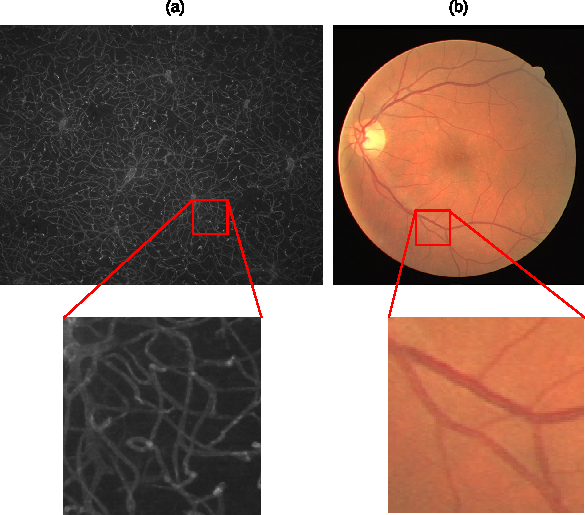
\includegraphics[width=\columnwidth]{figures/vessel_retinal_cortex.pdf}
    \caption{Illustration of the universality of vessel shape. (a) Fluorescence microscopy sample of a mouse cortex. (b) Fundus photograph of a human eye. Despite having different textures, the vessels have similar shapes.}
    \label{f:motivation}
\end{figure}

Based on this observation, we hypothesize that a model pretrained on a source domain with a strong shape bias will require only a few annotated samples to adapt to a new target domain. We expect such a model to outperform one trained from scratch in the target domain by effectively reusing its learned geometric priors. To test this hypothesis, we introduce VessShape, a large-scale synthetic dataset designed for pretraining shape-aware segmentation models. VessShape consists of 2D images with tubular, vessel-like structures paired with a wide variety of foreground and background textures. By fixing the geometric priors while diversifying the textures, the dataset explicitly encourages models to learn robust shape features over superficial texture cues.

In this work, we demonstrate that a model pretrained on VessShape achieves strong few-shot performance, accurately segmenting vasculature in different target domains using only four to ten annotated samples for fine-tuning. Furthermore, we observe remarkable zero-shot capabilities, where the pretrained model can effectively segment vessels in new domains without any target-specific training.

\section{Related Works}
\label{sec:related}

Many previous work has considered shape priors for medical image segmentation. This is possible when organelles, cells, or organs have a known shape and the segmentation process can assume an optimal shape or additional optimization criteria such as the requirement of smooth borders. Instance segmentation is probably the most common task in which shape priors have been explored. A particular challenge with blood vessel identification is that it usually requires a semantic segmentation of the image. 

Before the popularity of deep learning methods, local shape priors were the dominant approach to vessel segmentation. Blood vessels tend to have a tubular structure. Thus, the usual approach was to develop filters aimed at identifying tubular objects. A popular line of research was based on the eigenvalues of the Hessian matrix~\cite{fraz2012blood,sato1998three}. Arguably, the most popular Hessian-based method is the Frangi filter~\cite{frangi1998multiscale}, which consists of combining the eigenvalues to define a tubularity score for the pixels of the vessels. Another popular line of research was based on the definition of line or Gabor filter templates to identify relevant vessel structures. An important drawback of these methods is that the tubularity assumption is not valid at bifurcation and termination points.

With the emergence of deep learning, some works have explored adding shape priors during network training~\cite{bohlender2021survey}. Priors have been added on the network input using vesselness filters~\cite{affane2022robust,hu2024domain,garret2024deep}, on the network architecture using learnable vesselness or Gabor filters~\cite{chen2023learnable,fu2018frangi,volkov2025modification} and on the network output using topology-aware loss functions~\cite{shit2021cldice,hu2019topology,berger2024topologically}. For neural networks, it is simpler and likely more flexible to consider a data-based approach to add shape priors to the model. That is, to focus on generating a large and diverse set of images containing a priori knowledge regarding the structure of blood vessels. To our knowledge, no previous work tried to use the same method considered in our work. The closest approach is to generate synthetic images that are as similar as possible to the samples in the dataset. This has been done using two main strategies: i) using an appearance model of the vessels and image background~\cite{tetteh2020deepvesselnet,wittmann2025vesselfm,wittmann2024simulation,mathys2025synthetic} and ii) using style transfer or a generative model to create the samples. 

Modeling-based approaches usually start by generating a biologically plausible topology of the vasculature, followed by the definition of varying radii for vessel segments and the inclusion of texture for the vessels and the background. The typical noise found in the imaging modality of interest is also modeled. An important recent work in this direction is a foundation model called VesselFM~\cite{wittmann2025vesselfm} that was trained on a large number of synthetic and real images.

Regarding generative models, most works in the literature use inductive learning, applying Generative Adversarial Networks (GANs) to create samples~\cite{you2022application,andreini2021two,tavakkoli2020novel,costa2017end}. Synthetic samples conform to the learned patterns from the real dataset, allowing the generation of realistic images. Recent works considered diffusion models for the same task~\cite{go2024generation,guo2025vesseldiffusion,wang2025vastsd}. Some studies also developed style transfer approaches for domain adaptation between different datasets~\cite{peng2022unsupervised,chen2023segmentation,chen2021real}.

The main drawback of the aforementioned works is that the network is trained to reproduce the shape and texture of blood vessels in specific datasets. Changes in the texture of the vessels due to diseases or modifications in the imaging device can lead to low segmentation performance. In addition, models must be trained for specific imaging modalities, even if annotated data are scarce. Our approach aims at training neural networks to segment any vascular tissue that follows the shape priors acquired from VessShape.



\section{Methodology}
\label{s:methodology}

\subsection{The VessShape Dataset}

VessShape\footnote{{Dataset repository}: \url{https://github.com/galvaowesley/vess-shape-dataset}} defines the geometry of its synthetic images using Bézier curves, which allow a flexible and controlled representation of tubular shapes. Each vascular segment is described by an $n$th-order Bézier curve with control points $\{\mathbf{p}_i\}_{i=0}^n$. Segment tortuosity is adjusted by small perturbations to these control points, ensuring realistic and diverse vessel geometry. The Bézier curve $\mathbf{c}(t)$ of a vessel segment is given by Equation~\ref{eq:bezier}, where $t$ varies from 0 to 1.

\begin{equation}
\mathbf{c}(t) \,=\, \sum_{i=0}^{n} \binom{n}{i} (1-t)^{n-i} t^{i} \, \mathbf{p}_i,
\label{eq:bezier}
\end{equation}

To generate a curve, the first ($\mathbf{p}_0$) and last ($\mathbf{p}_n$) control points are randomly drawn with uniform probability. The remaining control points are generated by defining $n-2$ equally spaced points between a line connecting $\mathbf{p}_0$ and $\mathbf{p}_1$. Each of these points is then displaced by a random amount along a normal vector $\mathbf{n}_l$. This normal vector is a unit vector perpendicular to the line between $\mathbf{p}_0$ and $\mathbf{p}_1$. The displacement amount is drawn from a uniform distribution in $[-\delta,\delta]$. Lower values of $\delta$ lead to more straight curves.

For the generation of the binary mask $M$, each curve is discretized by sampling points at a sufficient resolution to capture its curvature, which are then sequentially connected to form a 1-pixel-thick polyline on the image grid. Subsequently, a binary morphological dilation with a disk-shaped structuring element of radius $r_0$ is applied, assigning a constant tubular thickness to the segments. 

To generate each binary mask, the number of segments $K$, the order $n$ of the Bézier curves, the displacement scale $\delta$ and the radius $r_0$ are all randomly sampled from an interval to ensure a wide variety of shapes. Table \ref{tab:vessshape_params} summarizes the parameters used in the VessShape dataset generation, along with their sampling ranges and descriptions.

\begin{table*}[t]
\caption{Main parameters used for generating the VessShape dataset.}
\label{tab:vessshape_params}
\centering
\begin{tabularx}{\textwidth}{l c X}
\hline
    \textbf{Parameter} & \textbf{Range} & \textbf{Description} \\
\hline
Number of curves $K$ & $[1,20]$ & Number of branches/vessels generated per sample. \\
Control points $n{+}1$ & $[2,20]$ & Bézier curve complexity (order $n$). \\
Displacement scale $\delta$ (px) & $[50.0,150.0]$ & Controls curvature/tortuosity via the typical amplitude of control-point displacement. \\
Initial radius $r_{0}$ (px) & $[1,5]$ & Basal vessel thickness; a smooth taper is applied along the branch. \\
Matting blur $\sigma$ & $[1,2]$ & Standard deviation of the Gaussian used for $A = G_{\sigma} * M$. \\

\hline
\end{tabularx}
\end{table*}

To compose the final image $I$ from a binary mask $M$, a foreground texture $F$ and a background texture $B$ are inserted into, respectively, the generated vessel segments and the background of the image. The textures are randomly selected from the ImageNet validation set \cite{JiaDeng2009}. Specifically, for each mask $M$, two images are randomly drawn from two distinct classes of the ImageNet dataset. The images are then randomly cropped and resized to the target dimensions ($H \times W$). An alpha matte $A$ is then generated by smoothing $M$ with a Gaussian filter of standard deviation $\sigma$ and normalizing its values to the $[0, 1]$ range. The textures are subsequently blended using this matte according to Equation \ref{eq:compose},

\begin{equation}
I \,=\, A\,F + (1-A)\,B,
\label{eq:compose}
\end{equation}

which ensures that vessel regions ($A \approx 1$) preserve the foreground while non-vessel regions ($A \approx 0$) retain the background. 

Parameter $\sigma$ controls the smoothness of the vessel boundaries. Examples of generated masks and images are shown in Figure~\ref{f:vessshape_sample}.


\begin{figure}[tbp]
    \centering
    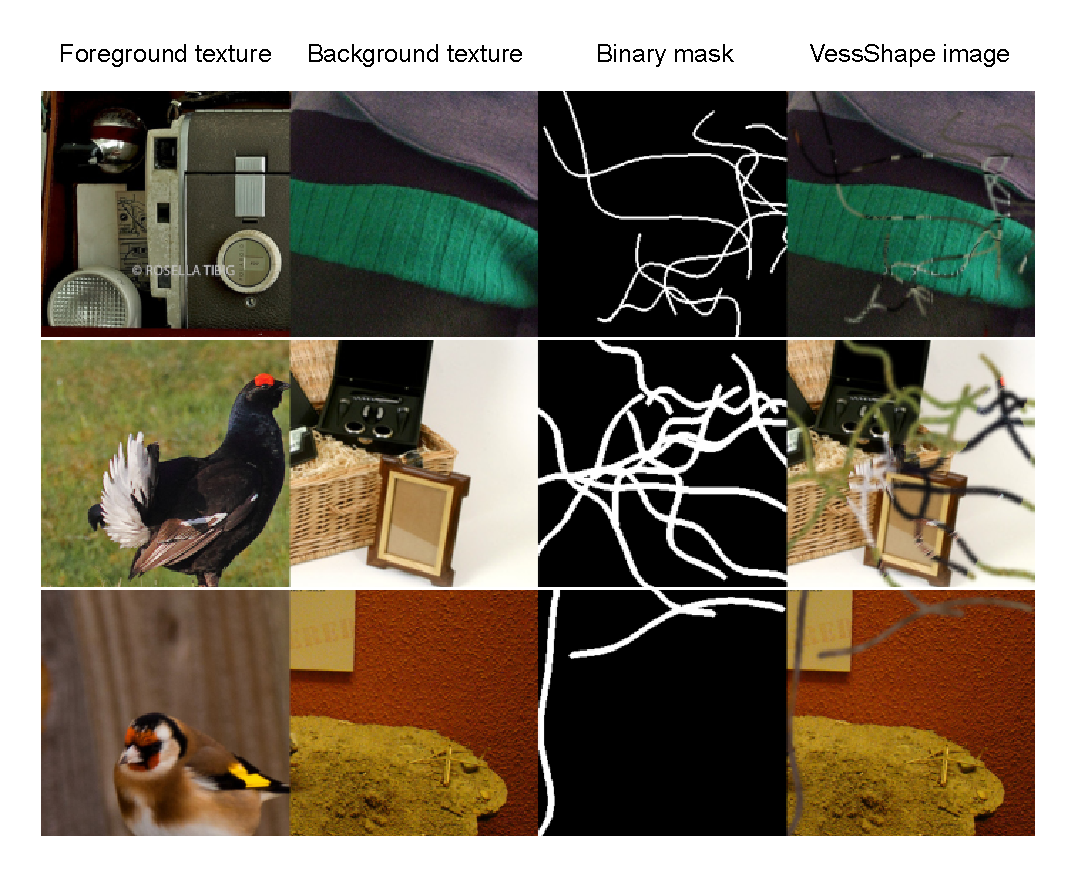
\includegraphics[width=\columnwidth]{figures/results/vessshape_sample.pdf}
    \caption{Examples of ImageNet samples, synthetic geometry and respective VessShape images. The ImageNet samples are used as textures for the synthetic binary masks, defining the respective VessShape image.}
    \label{f:vessshape_sample}
\end{figure}

\subsection{Real-world data for validation}

To quantify the usefulness of the shape bias introduced by the VessShape dataset, we consider two blood vessel datasets: DRIVE and VessMAP. The DRIVE dataset~\cite{Staal2004} serves as a popular standard for benchmarking retinal vessel segmentation algorithms and is composed of 40 fundus photographs split into 20 for training and 20 for testing, each measuring 584×565 pixels. The VessMAP dataset~\cite{viana2025new} consists of 100 images, 256×256 pixels each, acquired via fluorescence microscopy of the mouse cortex. It was curated to include a variety of challenging vascular features, such as inconsistent noise and contrast levels, different vessel sizes, prominent imaging artifacts, and intensity fluctuations within vessel structures.

The two datasets originate from fundamentally different imaging modalities, resulting in distinct characteristics. The fundus images in DRIVE, which capture the entire retina, possess a clear global structure that includes landmarks like the optic disk. The samples also contain many very thin vessels which are challenging to segment. In contrast, the VessMAP images are highly magnified views of small cortical areas and have no discernible global organization. The borders of the vessels are generally less defined than the vessels from DRIVE. Another key difference is that, without any processing, the vessels in VessMAP are bright with dark backgrounds while the vessels in DRIVE are dark with bright backgrounds. Figure \ref{f:drive_vessmap_samples} shows one sample from each dataset.

\begin{figure}[tbp]
    \centering
    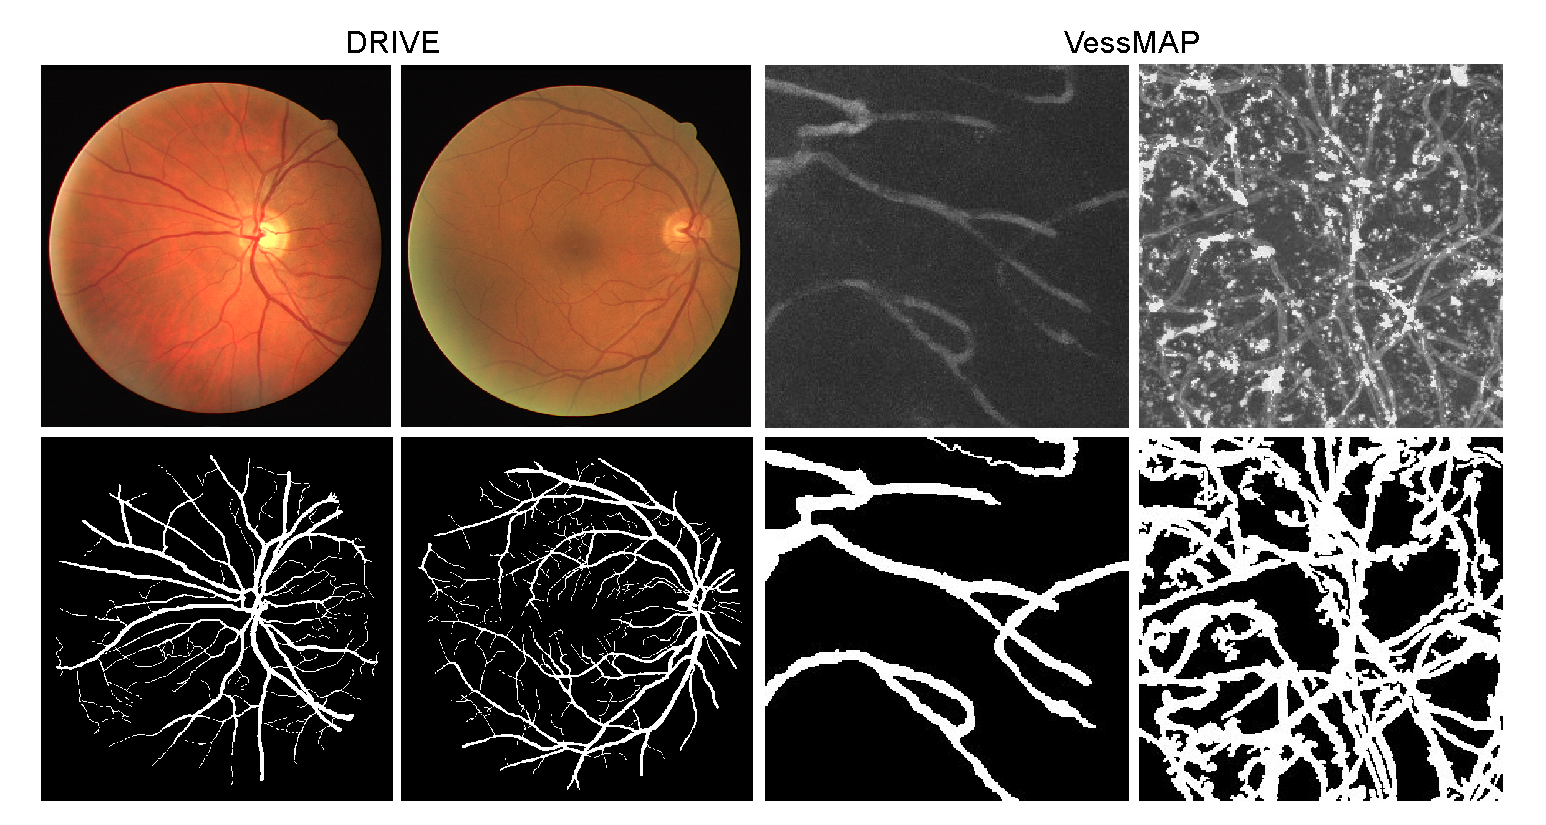
\includegraphics[width=\columnwidth]{figures/results/drive_vessmap_samples.pdf}
    \caption{Samples from the DRIVE and VessMAP datasets and their respective ground-truth masks.}
    \label{f:drive_vessmap_samples}
\end{figure}

\subsection{Model architectures and training strategies}

We adopt an encoder–decoder U-Net design, that is, the decoder is symmetrical to the encoder and the model contains skip connections between different encoder-decoder stages. Two models are compared, one with a ResNet18 and the other with a ResNet50 encoder \cite{he2016deep}. The models were instantiated from the \textit{Segmentation Models Pytorch} Python package\footnote{\url{https://github.com/qubvel/segmentation_models.pytorch}}.

Two training scenarios are considered. In the first, training is done from scratch separately on the DRIVE and VessMAP datasets to establish a baseline. The second scenario consists of pretraining on the VessShape dataset and fine-tuning on DRIVE and VessMAP to measure the transferability and sample efficiency of the learned representations. These two scenarios involve three distinct training procedures: i) pretraining on VessShape, ii) fine-tuning on real-world data and iii) training from scratch on real-world data. These procedures are described next.

\subsection{Pretraining on VessShape}

The pretraining on VessShape aims to expose the model to a wide variety of tubular geometries while keeping texture as a secondary cue. Each training sample is generated on-the-fly. This continual reshuffling of appearance paired with stable geometric rules should inject a strong shape bias while discouraging memorization of textures. The model is optimized to minimize the cross-entropy loss over this effectively unbound synthetic stream. 

We pre-train two U-Net models with ResNet18 and ResNet50 encoders, referred to as VSUNet18 and VSUNet50. VSUNet18 was exposed to about 7.1 million synthetic images in roughly 8.6 hours of training, and VSUNet50 to about 53.0 million in roughly 78.3 hours. Channel-wise normalization with ImageNet statistics was used for all input images. Table \ref{tab:vs_hparams} lists the hyperparameters used. Table~\ref{tab:vessshape_results} summarizes training performance on VessShape. All pretraining runs were executed on a workstation with 24 logical CPU cores and a single NVIDIA GeForce RTX 3090 GPU.

\begin{table}[t]
    \caption{Pretraining hyperparameters on VessShape.}
    \label{tab:vs_hparams}
    \centering
    \begingroup
    \small
    \setlength{\tabcolsep}{6pt}
    \renewcommand{\arraystretch}{1.15}
    \begin{tabular}{l r r}
        \hline
        	\textbf{Hyperparameter} & \textbf{VSUNet50} & \textbf{VSUNet18} \\
        \hline
        Batch size & 96 & 192 \\
        Learning rate & 1.0e-3 & 1.0e-2 \\
        Weight decay & 1.0e-4 & 0.0 \\
        \hline
    \end{tabular}
    \endgroup
\end{table}

\subsection{Fine-tuning}

We developed a systematic fine-tuning protocol\footnote{Code (VessShape pretraining + few-shot fine-tuning): \url{https://github.com/galvaowesley/vess-shape-experiments} } for few-shot training applicable to any 2D blood vessel dataset, but here applied to DRIVE and VessMAP. The goal is to quantify performance gains as the number of labeled examples used for adaptation increases. For the VSUNet variants, we always start from VessShape-pretrained weights.

For each dataset $D$ we split the images into three disjoint subsets: $\mathcal{V}_{\text{train}}$, the pool of labeled images eligible for few-shot sampling; $\mathcal{V}_{\text{val}}$, used for auxiliary adjustments; and $\mathcal{V}_{\text{test}}$, held out for final evaluation. For DRIVE we use 16 images in $\mathcal{V}_{\text{train}}$, 4 in $\mathcal{V}_{\text{val}}$, and keep 20 images in $\mathcal{V}_{\text{test}}$. For VessMAP we adopt 60 images for $\mathcal{V}_{\text{train}}$, 20 for $\mathcal{V}_{\text{val}}$, and 20 for $\mathcal{V}_{\text{test}}$.

To apply fine-tuning with progressive sampling we define an ordered set of sample sizes $\mathcal{N} = \{ n_1, n_2, \ldots, n_K \}$ with $n_1 = 1$ and $n_K = n_{\mathcal{V}_{\text{train}}}$. For each $n \in \mathcal{N}$ we perform $R$ independent runs, and for each run $r$ we sample without replacement a training subset:
\[
\mathcal{V}^{(n,r)}_{\text{train}} = \text{sample}(\mathcal{V}_{\text{train}}, n), \qquad \mathcal{V}^{(n,r)}_{\text{train}} \subseteq \mathcal{V}_{\text{train}}.
\]

For each $n$, we keep the set of already used samples and resample until obtaining a new combination or reaching a maximum number of attempts. If the combinatorial space is exhausted (for large $n$ or high $R$), repetition is allowed, ensuring training runs that are as diverse as possible.

Each subset $\mathcal{V}^{(n,r)}_{\text{train}}$ is used to fine-tune the model $S$ times ($s=1,\ldots,S$). The model is optimized to minimize the cros-entropy loss over $\mathcal{V}^{(n,r)}_{\text{train}}$, and performance is monitored on $\mathcal{V}_{\text{val}}$ after each epoch. The last checkpoint is then evaluated on $\mathcal{V}_{\text{test}}$. This approach allows decomposition of variance into: (i) training variability conditioned on a fixed image combination (within $(n,r)$) and (ii) variability across different image combinations between runs $r$.

In this work we set $R=5$ and $S=3$. The sample size sequences $\mathcal{N}$ are $\{1,2,4,8,16\}$ for DRIVE and $\{1,2,4,8,16,18,20\}$ for VessMAP. We also consider the zero-shot case ($n=0$), in which the pretrained model is evaluated directly on $\mathcal{V}_{\text{test}}$ without any adaptation on $D$. 

Additionally, we enforce reproducibility via a two-level seeding scheme: a deterministic seed derived from $(n,r)$ defines each training subset, which is then reused across $S$ stochastic repetitions differing only by a repetition seed


\subsection{Training from scratch on natural datasets}

In this stage we establish the baseline by training models directly on DRIVE and VessMAP without any synthetic pretraining. We denote these models U-Net18 and U-Net50, and the protocol mirrors, point by point, the fine-tuning procedure. The only structural difference relative to the previous protocol is the lack of VessShape-pretrained weights, which exposes the network to a noisier initial phase and one potentially more dependent on texture.

We do not define a zero-shot case for U-Net models because there is no useful prior state before observing at least one labeled image, thus the learning curve starts at $n=1$. The few-shot curves and the full-sample regime allow us to quantify: (i) the absolute gain provided by the shape bias acquired via VessShape; (ii) the difference in convergence speed as $n$ increases. In this way, the VSUNet versus U-Net comparison isolates the effect of shape bias while keeping all other factors controlled.


\section{Results}
\label{s:results}

\begin{table}[t]
    \caption{Performance of VSUNet variants after pretraining on VessShape.}
    \label{tab:vessshape_results}
    \centering
    \begingroup
    \small
    \setlength{\tabcolsep}{6pt}
    \renewcommand{\arraystretch}{1.15}
    \begin{tabular}{l r r}
        \hline
        	\textbf{Metric} & \textbf{VSUNet50} & \textbf{VSUNet18} \\
        \hline
        Dice & $0.861 \,\pm\, 0.022$ & $0.859 \,\pm\, 0.077$ \\
        Acc & $0.960 \,\pm\, 0.008$ & $0.956 \,\pm\, 0.037$ \\
        IoU & $0.758 \,\pm\, 0.032$ & $0.761 \,\pm\, 0.096$ \\
        Prec & $0.780 \,\pm\, 0.037$ & $0.774 \,\pm\, 0.096$ \\
        Rec & $0.964 \,\pm\, 0.012$ & $0.974 \,\pm\, 0.018$ \\
        \hline
    \end{tabular}
    \endgroup
\end{table}

\begin{figure*}[tbp]
    \centering
    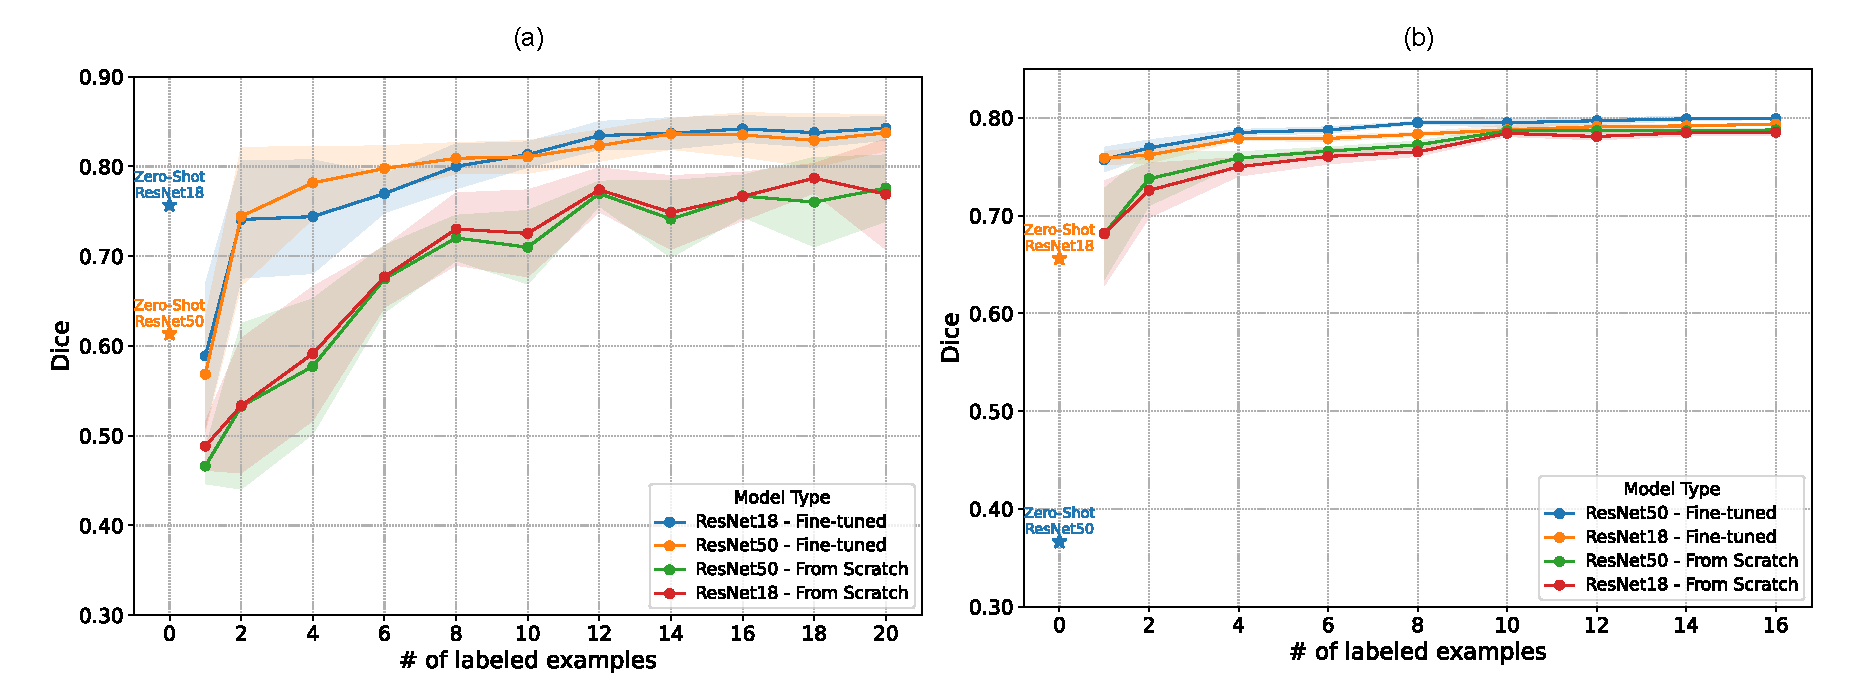
\includegraphics[width=\textwidth]{figures/results/results_charts.pdf}
    \caption{Few-shot and zero-shot Dice performance on (a) DRIVE and (b) VessMAP. Curves show the mean Dice over $R{=}5$ runs and $S{=}3$ repetitions for each sample size $n$; VessShape pretraining provides strong zero-shot ability for VessMAP, and faster saturation compared to training from scratch for both datasets. VSUNet variants outperform U-Net baselines at all cenarios, especially in the low-sample regime. The performance gap narrows at larger $n$ but remains non‑zero, indicating a persistent benefit from the learned shape bias.}
    \label{f:results_charts}
\end{figure*}


\begin{figure*}[tbp]
    \centering
    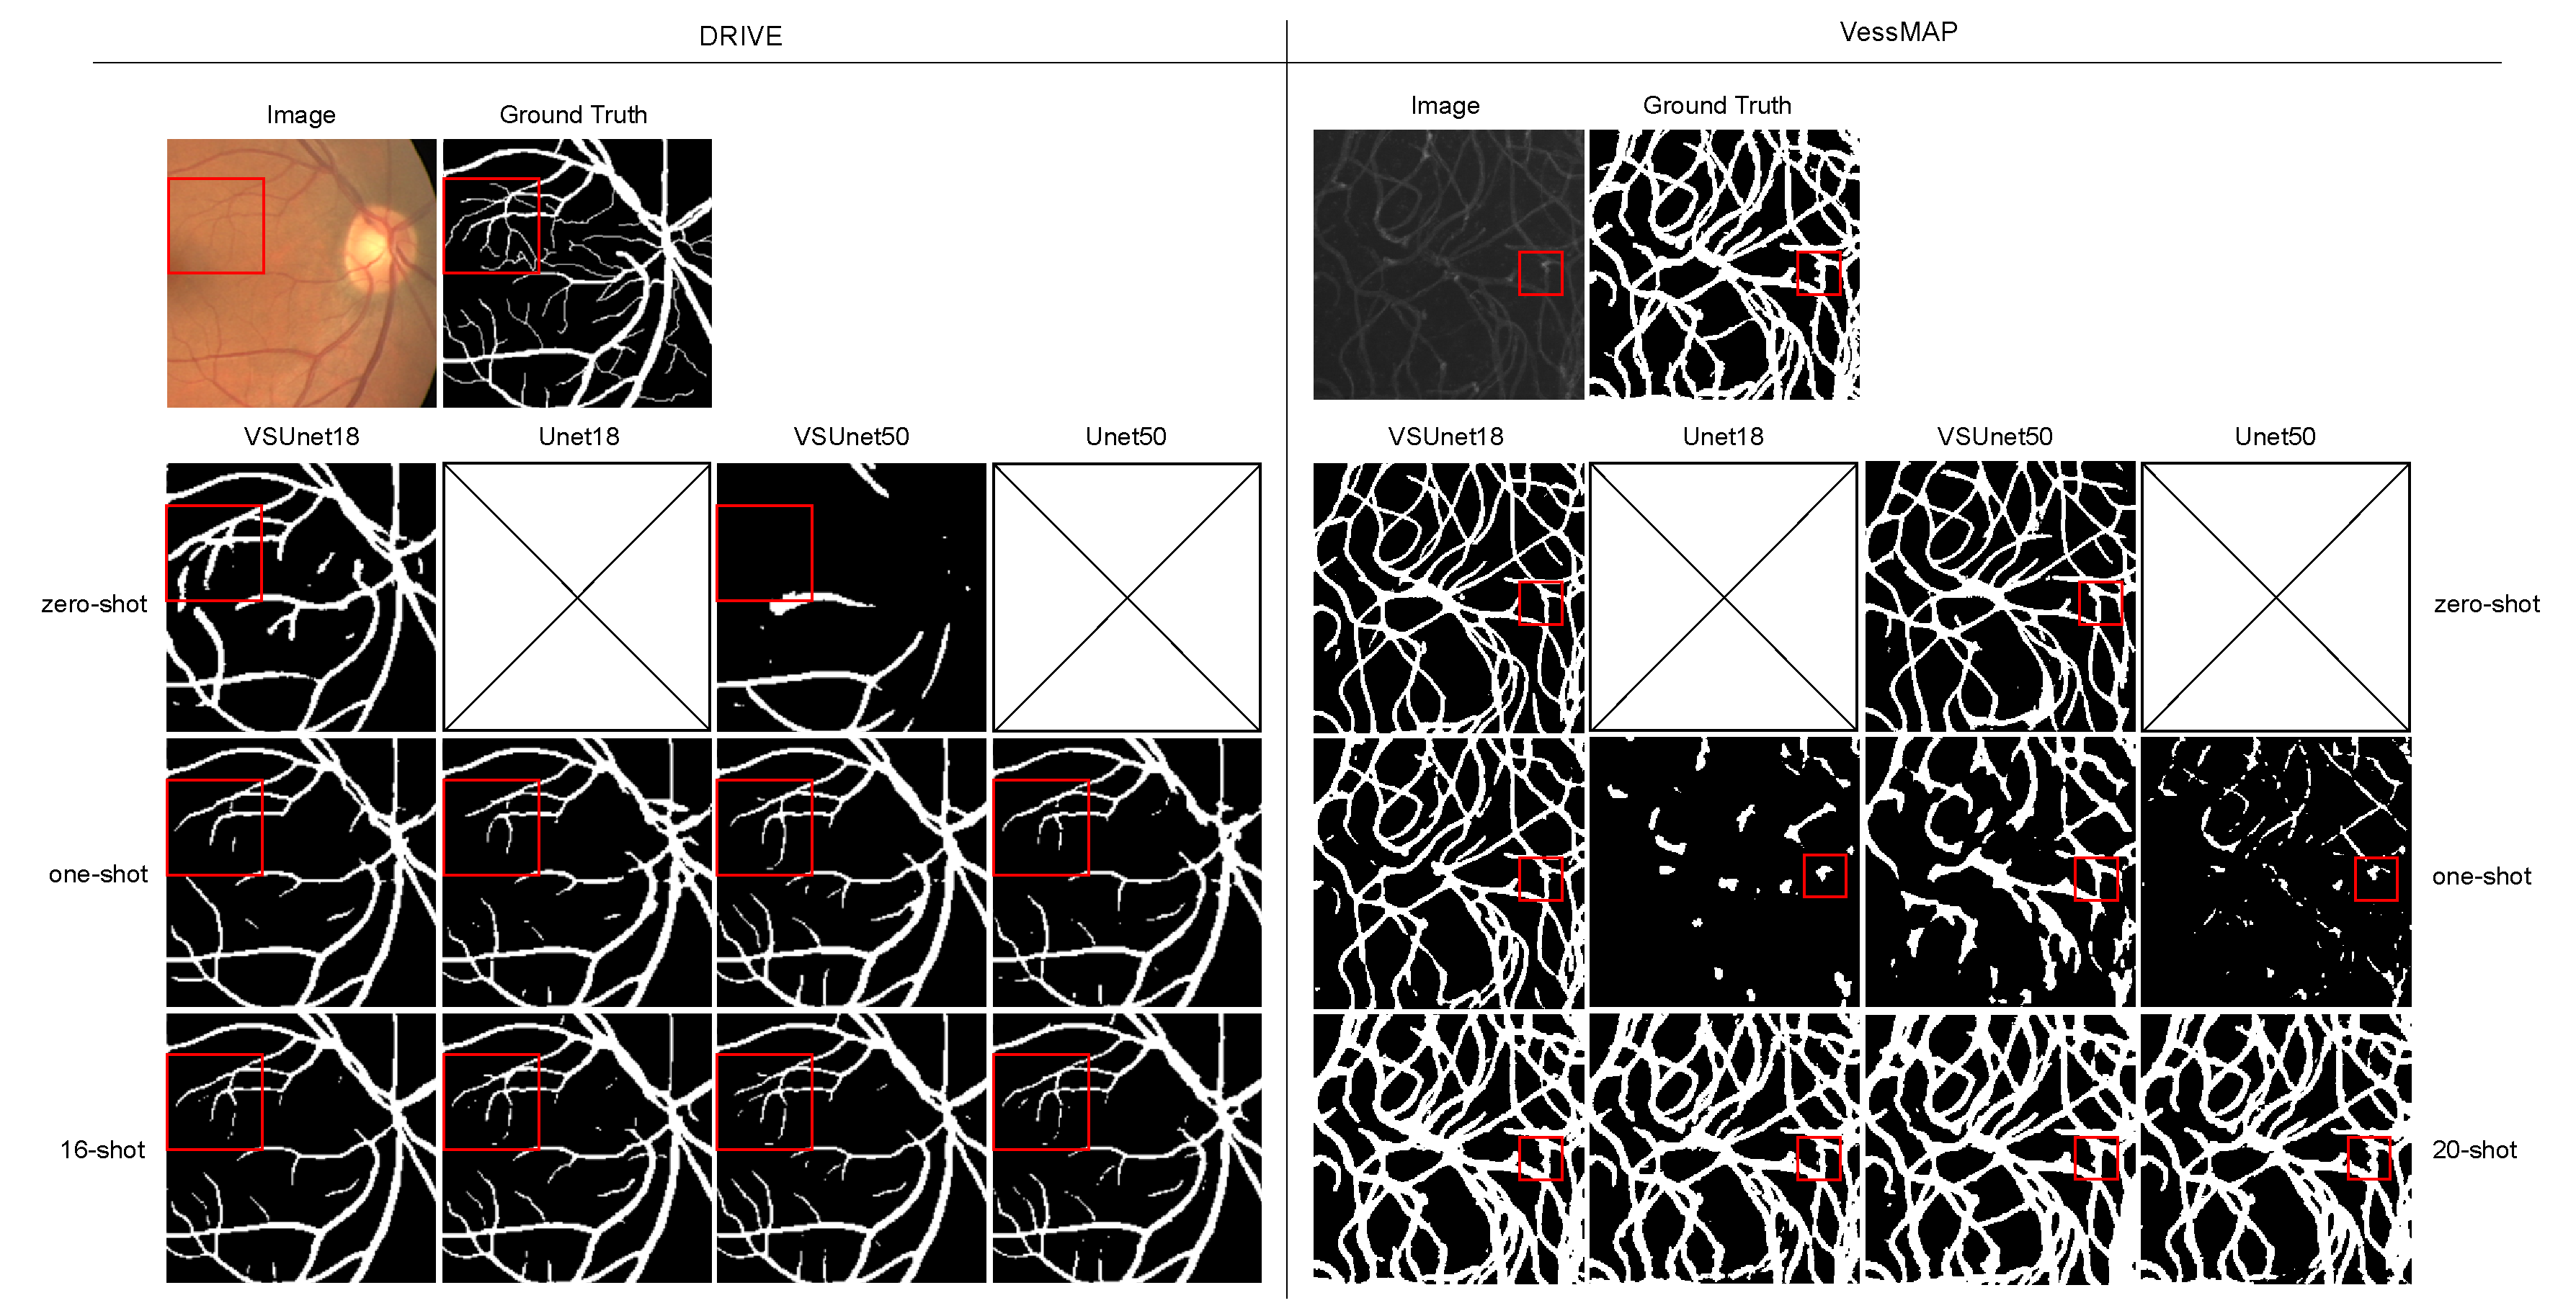
\includegraphics[width=\textwidth]{figures/results/results_fewshots.pdf}
    \caption{??.}
    \label{f:results_fewshots_drive}
\end{figure*}




% TODO:
% Argumentar que o nosso modelo é capaz de segmentar em zero-shot a forma do vaso, mesmo para VessMap que tem vasos com intensidade mais alta (branco), e DRIVE, com vasos com intensidade mais baixa(preto). 

% TODO: Testar trocando o número de exemplos como colunas, usando só o DICE. 
\begin{table*}[t]
    \caption{Few-shot and zero-shot segmentation on VessMAP and DRIVE. Values are mean $\pm$ standard deviation over repeated runs (fine-tuning for VSUNet models and training from scratch for U-Net baselines) evaluated on each dataset test set. Zero-shot rows come from a single pretrained inference (no deviation available).}
    \label{tab:combined_fewshot}
    \centering
    \begingroup
    \small
    \setlength{\tabcolsep}{4pt}
    \renewcommand{\arraystretch}{1.15}
    % Removed AUC column; merged Dataset cells with multirow
    \begin{tabular}{l r l r r r r r}
        \hline
        \textbf{Dataset} & \textbf{\#Examples} & \textbf{Model} & \textbf{Dice} & \textbf{Acc} & \textbf{IoU} & \textbf{Prec} & \textbf{Rec} \\
        \hline
        \multirow{10}{*}{DRIVE} & \multirow{2}{*}{0} & VSUNet18 & $0.656 \,\pm\, 0.000$ & $0.907 \,\pm\, 0.000$ & $0.490 \,\pm\, 0.000$ & $0.629 \,\pm\, 0.000$ & $0.699 \,\pm\, 0.000$ \\
         &  & VSUNet50 & $0.367 \,\pm\, 0.000$ & $0.888 \,\pm\, 0.000$ & $0.230 \,\pm\, 0.000$ & $0.728 \,\pm\, 0.000$ & $0.275 \,\pm\, 0.000$ \\
         \cline{2-8}
         & \multirow{4}{*}{1} & VSUNet18 & $0.759 \,\pm\, 0.007$ & $0.941 \,\pm\, 0.002$ & $0.612 \,\pm\, 0.009$ & $0.787 \,\pm\, 0.021$ & $0.741 \,\pm\, 0.019$ \\
         &  & VSUNet50 & $0.757 \,\pm\, 0.013$ & $0.939 \,\pm\, 0.006$ & $0.611 \,\pm\, 0.016$ & $0.773 \,\pm\, 0.046$ & $0.754 \,\pm\, 0.039$ \\
         &  & UNet18 & $0.682 \,\pm\, 0.054$ & $0.919 \,\pm\, 0.016$ & $0.523 \,\pm\, 0.058$ & $0.717 \,\pm\, 0.079$ & $0.690 \,\pm\, 0.118$ \\
         &  & UNet50 & $0.681 \,\pm\, 0.046$ & $0.916 \,\pm\, 0.031$ & $0.523 \,\pm\, 0.050$ & $0.722 \,\pm\, 0.099$ & $0.690 \,\pm\, 0.110$ \\
         \cline{2-8}
         & \multirow{4}{*}{16} & VSUNet18 & $0.794 \,\pm\, 0.000$ & $0.950 \,\pm\, 0.000$ & $0.658 \,\pm\, 0.000$ & $0.833 \,\pm\, 0.004$ & $0.762 \,\pm\, 0.003$ \\
         &  & VSUNet50 & $0.799 \,\pm\, 0.001$ & $0.952 \,\pm\, 0.000$ & $0.666 \,\pm\, 0.001$ & $0.846 \,\pm\, 0.003$ & $0.762 \,\pm\, 0.004$ \\
         &  & UNet18 & $0.785 \,\pm\, 0.003$ & $0.946 \,\pm\, 0.001$ & $0.647 \,\pm\, 0.004$ & $0.795 \,\pm\, 0.005$ & $0.781 \,\pm\, 0.004$ \\
         &  & UNet50 & $0.788 \,\pm\, 0.002$ & $0.947 \,\pm\, 0.001$ & $0.650 \,\pm\, 0.002$ & $0.807 \,\pm\, 0.006$ & $0.774 \,\pm\, 0.004$ \\
        \hline
        \multirow{10}{*}{VessMAP} & \multirow{2}{*}{0} & VSUNet18 & $0.757 \,\pm\, 0.000$ & $0.886 \,\pm\, 0.000$ & $0.616 \,\pm\, 0.000$ & $0.846 \,\pm\, 0.000$ & $0.696 \,\pm\, 0.000$ \\
         &  & VSUNet50 & $0.614 \,\pm\, 0.000$ & $0.817 \,\pm\, 0.000$ & $0.472 \,\pm\, 0.000$ & $0.746 \,\pm\, 0.000$ & $0.605 \,\pm\, 0.000$ \\
         \cline{2-8}
         & \multirow{4}{*}{1} & VSUNet18 & $0.589 \,\pm\, 0.080$ & $0.705 \,\pm\, 0.205$ & $0.455 \,\pm\, 0.088$ & $0.675 \,\pm\, 0.205$ & $0.738 \,\pm\, 0.148$ \\
         &  & VSUNet50 & $0.569 \,\pm\, 0.063$ & $0.708 \,\pm\, 0.203$ & $0.439 \,\pm\, 0.071$ & $0.683 \,\pm\, 0.208$ & $0.700 \,\pm\, 0.167$ \\
         &  & UNet18 & $0.488 \,\pm\, 0.027$ & $0.674 \,\pm\, 0.184$ & $0.362 \,\pm\, 0.032$ & $0.682 \,\pm\, 0.204$ & $0.622 \,\pm\, 0.210$ \\
         &  & UNet50 & $0.466 \,\pm\, 0.020$ & $0.665 \,\pm\, 0.181$ & $0.343 \,\pm\, 0.025$ & $0.674 \,\pm\, 0.206$ & $0.604 \,\pm\, 0.215$ \\
         \cline{2-8}
         & \multirow{4}{*}{20} & VSUNet18 & $0.843 \,\pm\, 0.013$ & $0.901 \,\pm\, 0.021$ & $0.739 \,\pm\, 0.018$ & $0.825 \,\pm\, 0.049$ & $0.888 \,\pm\, 0.048$ \\
         &  & VSUNet50 & $0.837 \,\pm\, 0.020$ & $0.905 \,\pm\, 0.025$ & $0.732 \,\pm\, 0.026$ & $0.851 \,\pm\, 0.032$ & $0.850 \,\pm\, 0.027$ \\
         &  & UNet18 & $0.769 \,\pm\, 0.062$ & $0.880 \,\pm\, 0.034$ & $0.645 \,\pm\, 0.075$ & $0.864 \,\pm\, 0.045$ & $0.737 \,\pm\, 0.094$ \\
         &  & UNet50 & $0.776 \,\pm\, 0.037$ & $0.880 \,\pm\, 0.035$ & $0.653 \,\pm\, 0.046$ & $0.855 \,\pm\, 0.041$ & $0.752 \,\pm\, 0.051$ \\
        \hline
    \end{tabular}
    \endgroup
\end{table*}



\section{Conclusion}
\label{s:conclusion}

We proposed a strategy centered on instilling a strong shape bias in deep learning models by pretraining them on VessShape, a large-scale synthetic dataset. By combining simple, universal vessel-like geometries with highly diverse textures, VessShape encourages models to learn robust shape priors instead of domain-specific texture features.

Our experiments demonstrated the effectiveness of this approach. A model pretrained on VessShape achieved strong few-shot performance on two distinct and challenging real-world datasets, DRIVE (retinal fundus photography) and VessMAP (cerebral cortex microscopy), requiring only a handful of annotated samples to adapt to these new domains. Furthermore, the model exhibited remarkable zero-shot capabilities, successfully identifying vessel structures without any fine-tuning. These results confirm our hypothesis that the use of a fundamental geometric prior is a powerful method to improve data efficiency and model robustness against domain shifts.

Although our method shows significant promise, there are avenues for future work. The current geometry generation in VessShape, based on Bézier curves, could be extended to include more complex and biologically plausible vascular topologies, such as true bifurcations and network-like structures. Furthermore, extending the VessShape generation framework to 3D would allow this pretraining strategy to be applied to volumetric medical imaging modalities such as CT and MRI. Future studies could also explore the application of a shape-centric pretraining approach to the segmentation of other tubular structures in biology, such as neurons or airways.

Our work underscores a valuable principle: for segmentation tasks with strong and consistent shape priors, abstracting away from realism to focus on core geometric features can be a more effective and generalizable pretraining strategy than attempting to perfectly mimic the appearance of a single target domain.


% One drawback of the method is that the network might not recognize vessels that do not follow the shape priors acquiried during training. For instance, stroke....


\section*{Funding}
C. H. Comin thanks FAPESP (grant no. 21/12354-8) for financial support. 


\bibliography{references}

\end{document}